\documentclass{IEEEtran}

\hbadness=999999

% Packages
\usepackage{amsmath}
\usepackage{physics}
\usepackage[cmintegrals]{newtxmath}
\usepackage{graphicx}
\usepackage{xurl} % Makes urls better
\usepackage{caption}
\graphicspath{{./images}}


% Title Stuff
\title{Experiment 5: Starting Torque of Induction Motors}
\author{Chase Lotito, Blake Jourdan, Noah Holland}
\date{}

% Begin document
\begin{document}

% Make the title
\maketitle

% ABSTRACT
\begin{abstract}
    % [A brief statement on what you plan to do in this project.]
    The following experiment acquainted us with the induction motor, specifically how to find the starting torque of an IM-100 induction motor. Using a DYN-100-DM dynamometer with a clamp to lock the rotor, this emulates the starting of a motor. The experiment shows the large inrush currents motors experience, a starting torque larger than running torque, and a poor power factor \(pf\approx 0.622\).  
\end{abstract}

\section{Introduction}

The following experiment was followed as described in the lab manual \cite{labmanual}. However, a slight deviation was made with the measurement of active power consumed by the induction motor. Since the second wattmeter on the Hampden Console (Fig. \ref{fig:console}) was broken, the 2-wattmeter method could not be used; instead, power was measured at a single phase from line-to-neutral and the total power is triple that.


\begin{figure}[h!]
    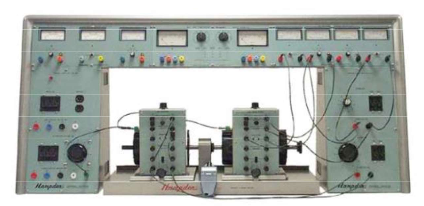
\includegraphics[width=\columnwidth]{console.png}
    \caption{Hampden Console}
    \centering
    \label{fig:console}
\end{figure}

The experiment performed was locked-rotor test. The rotor was locked by coupling the shaft of the dynamometer to the motor shaft and then mechanically clamping the dynamometer shaft (Fig \ref{fig:coupled}).

\begin{figure}[h!]
    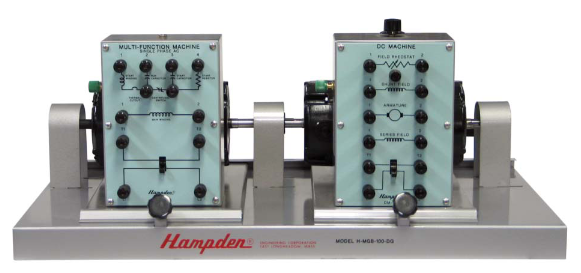
\includegraphics[width=\columnwidth]{coupled.png}
    \caption{Coupled Induction Machine and Dynamometer}
    \centering
    \label{fig:coupled}
\end{figure}

From there, an ammeter and voltmeter were connected to a single stator phase, and the wattmeter was connected from line-to-neutral. Then the motor was energized at 104V (half nominal) for a few seconds to measure inrush current, voltage level, active power, and starting torque. Torque was measured with the Hampden H-REM-LC-D signal conditioner (Fig. \ref{fig:torque}).

\begin{figure}[h!]
    \centering
    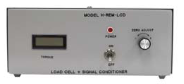
\includegraphics[width=0.5\columnwidth]{torque.png}
    \caption{Signal Conditioner}
    \label{fig:torque}
\end{figure}

\section{Debriefing}

The results from the experiment are found in Fig.\ref{fig:table1}-\ref{fig:table3}. Since power was measured from line-to-neutral \(P_{\text{line}}\), the total power \(P_{\text{total}}\)  was found as follows:

\begin{equation}
    P_{\text{total}} = 3P_{\text{line}}
\end{equation}

\begin{figure}[h!]
    
\includegraphics[width=\columnwidth]{table1.png}
    \caption{Experimental Data}
    \centering
    \label{fig:table1}
\end{figure}

We ran the locked-rotor test at half nominal voltage, so to calculate for torque at nominal voltage, we leverage that \(T\propto V^2\), so:

\begin{equation}
    T_{\text{full-voltage}} = 4 T_{\text{half-voltage}}
\end{equation}

Also, current is doubled at full voltage. From this, we can compute how much larger the inrush current to the motor is compared to the standard nominal current at speed:

\begin{equation}
    \frac{I_{\text{starting}}}{I_{\text{Running}}} \% = \frac{8}{1.4} \times 100 \% = 571\%
\end{equation}

Inrush current between 5-6 times larger than nominal current is textbook for an induction motor.

\begin{figure}[h!]
    
\includegraphics[width=\columnwidth]{table2.png}
    \caption{Starting vs. Running Characteristics}
    \centering
    \label{fig:table2}
\end{figure}

Using the line current and line voltage from Fig. \ref{fig:table1}, we can calculate the apparent power \(|S|\):

\begin{equation}
    |S| = \sqrt{3}VI = \sqrt{3}(104)(4) = 720.533 ~ \text{VA}
\end{equation}

Then using the active power measured in Fig. \ref{fig:table1} \(P=448\) W, the power factor \(pf\) can be calculated:

\begin{equation}
    pf = \frac{P}{|S|} = \frac{448}{720.533} = 0.622    
\end{equation}

Then we can easily find the power factor angle \(\varphi\) by using the inverse cosine of the power factor. Ultimately we find that the induction motor at start has a poor power factor since the rotor inductance is maximum at the beginnging \cite{labmanual}.

\begin{figure}[h!]
    
\includegraphics[width=\columnwidth]{table3.png}
    \caption{Apparent Power and Power Factor}
    \centering
    \label{fig:table3}
\end{figure}

From Experiment 4, where the motor was exposed to a variable load, we found that motor torque increased with increasing current \cite{lab4}, which we also see in this experiment a current 571\% larger than running current is a decent 4.013 N\(\cdot\)m, as compared to torques between 1-1.5 N\(\cdot\)m at near synchronous speed. 

For the variable load, in Lab 4, we found the motor torque to increase as power factor approached unity, but this does not contradict the large current we found for a poor power factor, since the rotor reactance would decrease as the motor got to speed, improving power factor, and moving the torque to the breakdown point as slip goes from 1 to nominal. 

Also, we see that our starting torque at \(T_{ST}=4.013\) N\(\cdot\)m is larger than running torque at \(T_{FL}=1.36\) N\(\cdot\)m , which should be expected as the running torque is past the maximum breakdown torque. Which is to be expected based on the charactersitic induction motor torque curve. 

\section{Conclusion}

Overall, the locked-rotor test performed validated much of the theoretical work done in ECE385. The inrush current we suspected to be large was 5 to 6 times larger than nominal current as expected, and we can see the poor power factor that results from that. Also, we can see that the motor torque was larger than nominal, but not as large as it could be as power factor would correct itself during operation.

% REFERENCES!
\bibliographystyle{IEEEtran}
\bibliography{bib.bib}

\end{document}
